\documentclass[tikz,border=2mm]{standalone}
\usepackage[utf8]{inputenc}
\usepackage[T1]{fontenc}
\usepackage{tikz}
\usetikzlibrary{arrows.meta, positioning}
\usepackage{pgfplots}

\pgfplotsset{compat=1.18}

\begin{document}

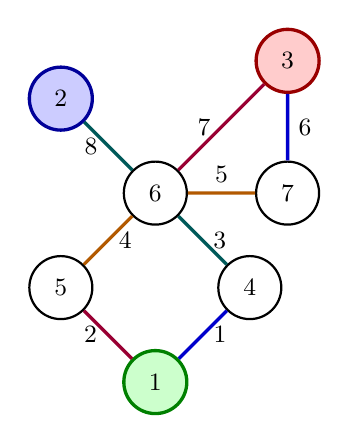
\begin{tikzpicture}[
  scale=1.2,
  every node/.style={font=\small},
  v/.style={circle, draw, thick, minimum size=8mm, inner sep=0pt},
  start/.style={v, fill=green!20, draw=green!50!black, very thick},
  exit/.style={v, fill=blue!20, draw=blue!60!black, very thick},
  rat/.style={v, fill=red!20, draw=red!60!black, very thick},
  pairA/.style={very thick, draw=blue!80!black},
  pairB/.style={very thick, draw=purple!80!black},
  pairC/.style={very thick, draw=teal!70!black},
  pairD/.style={very thick, draw=orange!70!black}
]

% Nodes
\node[start] (1) at (0,0) {1};
\node[v]     (4) at (1,1) {4};
\node[v]     (5) at (-1,1) {5};
\node[v]     (6) at (0,2) {6};
\node[v]     (7) at (1.4,2) {7};
\node[rat]   (3) at (1.4,3.4) {3};
\node[exit]  (2) at (-1,3) {2};

% Pair A: edges 1 & 6
\draw[pairA] (1) -- node[right] {1} (4);
\draw[pairA] (7) -- node[right] {6} (3);

% Pair B: edges 2 & 7
\draw[pairB] (1) -- node[left] {2} (5);
\draw[pairB] (3) -- node[left] {7} (6);

% Pair C: edges 3 & 8
\draw[pairC] (4) -- node[right] {3} (6);
\draw[pairC] (6) -- node[left] {8} (2);

% Pair D: edges 4 & 5
\draw[pairD] (5) -- node[right] {4} (6);
\draw[pairD] (6) -- node[above] {5} (7);

\end{tikzpicture}

\end{document}
